%\documentclass{standalone}
%\usepackage{tikz}
%\usetikzlibrary{patterns,plotmarks}
%\begin{document}
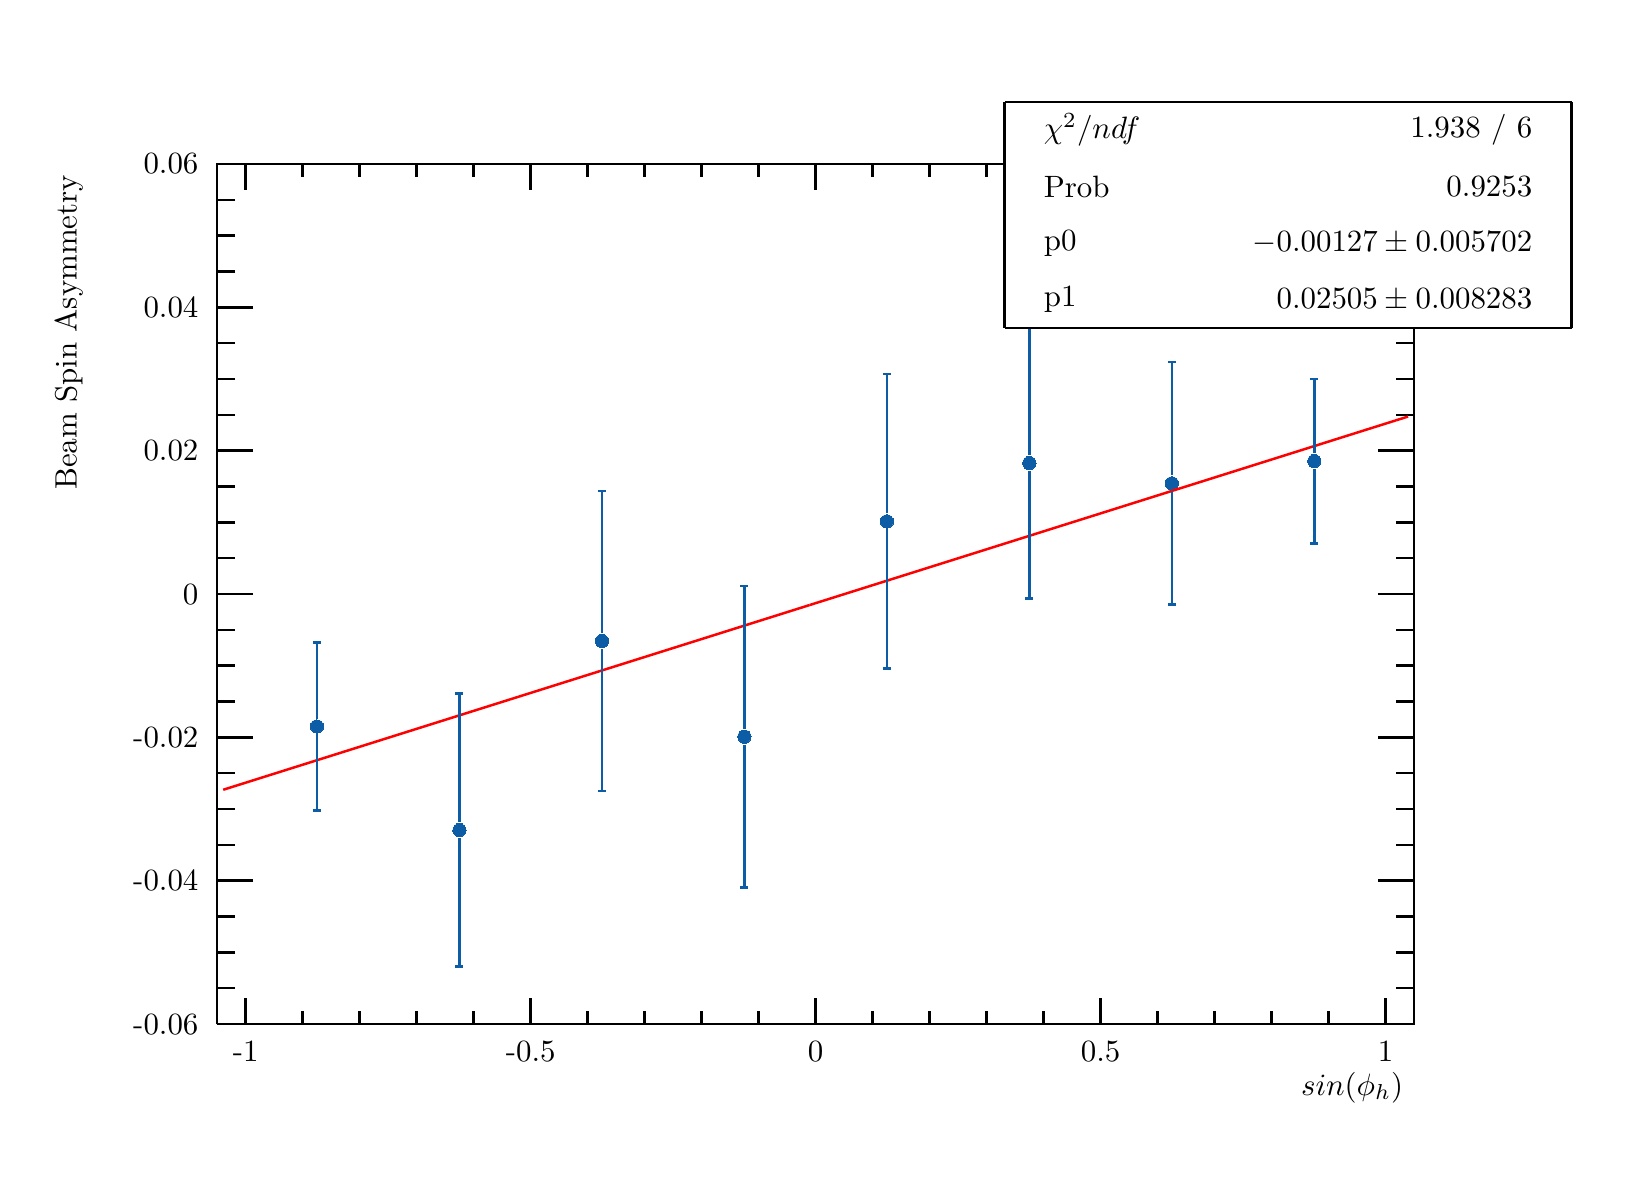
\begin{tikzpicture}
\def\CheckTikzLibraryLoaded#1{ \ifcsname tikz@library@#1@loaded\endcsname \else \PackageWarning{tikz}{usetikzlibrary{#1} is missing in the preamble.} \fi }
\CheckTikzLibraryLoaded{patterns}
\CheckTikzLibraryLoaded{plotmarks}
\pgfdeclareplotmark{cross} {
\pgfpathmoveto{\pgfpoint{-0.3\pgfplotmarksize}{\pgfplotmarksize}}
\pgfpathlineto{\pgfpoint{+0.3\pgfplotmarksize}{\pgfplotmarksize}}
\pgfpathlineto{\pgfpoint{+0.3\pgfplotmarksize}{0.3\pgfplotmarksize}}
\pgfpathlineto{\pgfpoint{+1\pgfplotmarksize}{0.3\pgfplotmarksize}}
\pgfpathlineto{\pgfpoint{+1\pgfplotmarksize}{-0.3\pgfplotmarksize}}
\pgfpathlineto{\pgfpoint{+0.3\pgfplotmarksize}{-0.3\pgfplotmarksize}}
\pgfpathlineto{\pgfpoint{+0.3\pgfplotmarksize}{-1.\pgfplotmarksize}}
\pgfpathlineto{\pgfpoint{-0.3\pgfplotmarksize}{-1.\pgfplotmarksize}}
\pgfpathlineto{\pgfpoint{-0.3\pgfplotmarksize}{-0.3\pgfplotmarksize}}
\pgfpathlineto{\pgfpoint{-1.\pgfplotmarksize}{-0.3\pgfplotmarksize}}
\pgfpathlineto{\pgfpoint{-1.\pgfplotmarksize}{0.3\pgfplotmarksize}}
\pgfpathlineto{\pgfpoint{-0.3\pgfplotmarksize}{0.3\pgfplotmarksize}}
\pgfpathclose
\pgfusepathqstroke
}
\pgfdeclareplotmark{cross*} {
\pgfpathmoveto{\pgfpoint{-0.3\pgfplotmarksize}{\pgfplotmarksize}}
\pgfpathlineto{\pgfpoint{+0.3\pgfplotmarksize}{\pgfplotmarksize}}
\pgfpathlineto{\pgfpoint{+0.3\pgfplotmarksize}{0.3\pgfplotmarksize}}
\pgfpathlineto{\pgfpoint{+1\pgfplotmarksize}{0.3\pgfplotmarksize}}
\pgfpathlineto{\pgfpoint{+1\pgfplotmarksize}{-0.3\pgfplotmarksize}}
\pgfpathlineto{\pgfpoint{+0.3\pgfplotmarksize}{-0.3\pgfplotmarksize}}
\pgfpathlineto{\pgfpoint{+0.3\pgfplotmarksize}{-1.\pgfplotmarksize}}
\pgfpathlineto{\pgfpoint{-0.3\pgfplotmarksize}{-1.\pgfplotmarksize}}
\pgfpathlineto{\pgfpoint{-0.3\pgfplotmarksize}{-0.3\pgfplotmarksize}}
\pgfpathlineto{\pgfpoint{-1.\pgfplotmarksize}{-0.3\pgfplotmarksize}}
\pgfpathlineto{\pgfpoint{-1.\pgfplotmarksize}{0.3\pgfplotmarksize}}
\pgfpathlineto{\pgfpoint{-0.3\pgfplotmarksize}{0.3\pgfplotmarksize}}
\pgfpathclose
\pgfusepathqfillstroke
}
\pgfdeclareplotmark{newstar} {
\pgfpathmoveto{\pgfqpoint{0pt}{\pgfplotmarksize}}
\pgfpathlineto{\pgfqpointpolar{44}{0.5\pgfplotmarksize}}
\pgfpathlineto{\pgfqpointpolar{18}{\pgfplotmarksize}}
\pgfpathlineto{\pgfqpointpolar{-20}{0.5\pgfplotmarksize}}
\pgfpathlineto{\pgfqpointpolar{-54}{\pgfplotmarksize}}
\pgfpathlineto{\pgfqpointpolar{-90}{0.5\pgfplotmarksize}}
\pgfpathlineto{\pgfqpointpolar{234}{\pgfplotmarksize}}
\pgfpathlineto{\pgfqpointpolar{198}{0.5\pgfplotmarksize}}
\pgfpathlineto{\pgfqpointpolar{162}{\pgfplotmarksize}}
\pgfpathlineto{\pgfqpointpolar{134}{0.5\pgfplotmarksize}}
\pgfpathclose
\pgfusepathqstroke
}
\pgfdeclareplotmark{newstar*} {
\pgfpathmoveto{\pgfqpoint{0pt}{\pgfplotmarksize}}
\pgfpathlineto{\pgfqpointpolar{44}{0.5\pgfplotmarksize}}
\pgfpathlineto{\pgfqpointpolar{18}{\pgfplotmarksize}}
\pgfpathlineto{\pgfqpointpolar{-20}{0.5\pgfplotmarksize}}
\pgfpathlineto{\pgfqpointpolar{-54}{\pgfplotmarksize}}
\pgfpathlineto{\pgfqpointpolar{-90}{0.5\pgfplotmarksize}}
\pgfpathlineto{\pgfqpointpolar{234}{\pgfplotmarksize}}
\pgfpathlineto{\pgfqpointpolar{198}{0.5\pgfplotmarksize}}
\pgfpathlineto{\pgfqpointpolar{162}{\pgfplotmarksize}}
\pgfpathlineto{\pgfqpointpolar{134}{0.5\pgfplotmarksize}}
\pgfpathclose
\pgfusepathqfillstroke
}
\definecolor{c}{rgb}{1,1,1};
\draw [color=c, fill=c] (0,0) rectangle (20,14.3719);
\draw [color=c, fill=c] (2.4,1.72462) rectangle (17.6,12.6472);
\definecolor{c}{rgb}{0,0,0};
\draw [c,line width=0.9] (2.4,1.72462) -- (2.4,12.6472) -- (17.6,12.6472) -- (17.6,1.72462) -- (2.4,1.72462);
\definecolor{c}{rgb}{1,1,1};
\draw [color=c, fill=c] (2.4,1.72462) rectangle (17.6,12.6472);
\definecolor{c}{rgb}{0,0,0};
\draw [c,line width=0.9] (2.4,1.72462) -- (2.4,12.6472) -- (17.6,12.6472) -- (17.6,1.72462) -- (2.4,1.72462);
\draw [c,line width=0.9] (2.4,1.72462) -- (17.6,1.72462);
\draw [c,line width=0.9] (2.7619,2.0523) -- (2.7619,1.72462);
\draw [c,line width=0.9] (3.48571,1.88846) -- (3.48571,1.72462);
\draw [c,line width=0.9] (4.20952,1.88846) -- (4.20952,1.72462);
\draw [c,line width=0.9] (4.93333,1.88846) -- (4.93333,1.72462);
\draw [c,line width=0.9] (5.65714,1.88846) -- (5.65714,1.72462);
\draw [c,line width=0.9] (6.38095,2.0523) -- (6.38095,1.72462);
\draw [c,line width=0.9] (7.10476,1.88846) -- (7.10476,1.72462);
\draw [c,line width=0.9] (7.82857,1.88846) -- (7.82857,1.72462);
\draw [c,line width=0.9] (8.55238,1.88846) -- (8.55238,1.72462);
\draw [c,line width=0.9] (9.27619,1.88846) -- (9.27619,1.72462);
\draw [c,line width=0.9] (10,2.0523) -- (10,1.72462);
\draw [c,line width=0.9] (10.7238,1.88846) -- (10.7238,1.72462);
\draw [c,line width=0.9] (11.4476,1.88846) -- (11.4476,1.72462);
\draw [c,line width=0.9] (12.1714,1.88846) -- (12.1714,1.72462);
\draw [c,line width=0.9] (12.8952,1.88846) -- (12.8952,1.72462);
\draw [c,line width=0.9] (13.619,2.0523) -- (13.619,1.72462);
\draw [c,line width=0.9] (14.3429,1.88846) -- (14.3429,1.72462);
\draw [c,line width=0.9] (15.0667,1.88846) -- (15.0667,1.72462);
\draw [c,line width=0.9] (15.7905,1.88846) -- (15.7905,1.72462);
\draw [c,line width=0.9] (16.5143,1.88846) -- (16.5143,1.72462);
\draw [c,line width=0.9] (17.2381,2.0523) -- (17.2381,1.72462);
\draw [c,line width=0.9] (2.7619,2.0523) -- (2.7619,1.72462);
\draw [c,line width=0.9] (17.2381,2.0523) -- (17.2381,1.72462);
\draw [anchor=base] (2.7619,1.25035) node[scale=1.11607, color=c, rotate=0]{-1};
\draw [anchor=base] (6.38095,1.25035) node[scale=1.11607, color=c, rotate=0]{-0.5};
\draw [anchor=base] (10,1.25035) node[scale=1.11607, color=c, rotate=0]{0};
\draw [anchor=base] (13.619,1.25035) node[scale=1.11607, color=c, rotate=0]{0.5};
\draw [anchor=base] (17.2381,1.25035) node[scale=1.11607, color=c, rotate=0]{1};
\draw [anchor= east] (17.6,0.919799) node[scale=1.11607, color=c, rotate=0]{$sin(\phi_{h})$};
\draw [c,line width=0.9] (2.4,12.6472) -- (17.6,12.6472);
\draw [c,line width=0.9] (2.7619,12.3196) -- (2.7619,12.6472);
\draw [c,line width=0.9] (3.48571,12.4834) -- (3.48571,12.6472);
\draw [c,line width=0.9] (4.20952,12.4834) -- (4.20952,12.6472);
\draw [c,line width=0.9] (4.93333,12.4834) -- (4.93333,12.6472);
\draw [c,line width=0.9] (5.65714,12.4834) -- (5.65714,12.6472);
\draw [c,line width=0.9] (6.38095,12.3196) -- (6.38095,12.6472);
\draw [c,line width=0.9] (7.10476,12.4834) -- (7.10476,12.6472);
\draw [c,line width=0.9] (7.82857,12.4834) -- (7.82857,12.6472);
\draw [c,line width=0.9] (8.55238,12.4834) -- (8.55238,12.6472);
\draw [c,line width=0.9] (9.27619,12.4834) -- (9.27619,12.6472);
\draw [c,line width=0.9] (10,12.3196) -- (10,12.6472);
\draw [c,line width=0.9] (10.7238,12.4834) -- (10.7238,12.6472);
\draw [c,line width=0.9] (11.4476,12.4834) -- (11.4476,12.6472);
\draw [c,line width=0.9] (12.1714,12.4834) -- (12.1714,12.6472);
\draw [c,line width=0.9] (12.8952,12.4834) -- (12.8952,12.6472);
\draw [c,line width=0.9] (13.619,12.3196) -- (13.619,12.6472);
\draw [c,line width=0.9] (14.3429,12.4834) -- (14.3429,12.6472);
\draw [c,line width=0.9] (15.0667,12.4834) -- (15.0667,12.6472);
\draw [c,line width=0.9] (15.7905,12.4834) -- (15.7905,12.6472);
\draw [c,line width=0.9] (16.5143,12.4834) -- (16.5143,12.6472);
\draw [c,line width=0.9] (17.2381,12.3196) -- (17.2381,12.6472);
\draw [c,line width=0.9] (2.7619,12.3196) -- (2.7619,12.6472);
\draw [c,line width=0.9] (17.2381,12.3196) -- (17.2381,12.6472);
\draw [c,line width=0.9] (2.4,1.72462) -- (2.4,12.6472);
\draw [c,line width=0.9] (2.856,1.72462) -- (2.4,1.72462);
\draw [c,line width=0.9] (2.628,2.17973) -- (2.4,2.17973);
\draw [c,line width=0.9] (2.628,2.63484) -- (2.4,2.63484);
\draw [c,line width=0.9] (2.628,3.08995) -- (2.4,3.08995);
\draw [c,line width=0.9] (2.856,3.54506) -- (2.4,3.54506);
\draw [c,line width=0.9] (2.628,4.00017) -- (2.4,4.00017);
\draw [c,line width=0.9] (2.628,4.45528) -- (2.4,4.45528);
\draw [c,line width=0.9] (2.628,4.91039) -- (2.4,4.91039);
\draw [c,line width=0.9] (2.856,5.36549) -- (2.4,5.36549);
\draw [c,line width=0.9] (2.628,5.8206) -- (2.4,5.8206);
\draw [c,line width=0.9] (2.628,6.27571) -- (2.4,6.27571);
\draw [c,line width=0.9] (2.628,6.73082) -- (2.4,6.73082);
\draw [c,line width=0.9] (2.856,7.18593) -- (2.4,7.18593);
\draw [c,line width=0.9] (2.628,7.64104) -- (2.4,7.64104);
\draw [c,line width=0.9] (2.628,8.09615) -- (2.4,8.09615);
\draw [c,line width=0.9] (2.628,8.55126) -- (2.4,8.55126);
\draw [c,line width=0.9] (2.856,9.00637) -- (2.4,9.00637);
\draw [c,line width=0.9] (2.628,9.46147) -- (2.4,9.46147);
\draw [c,line width=0.9] (2.628,9.91658) -- (2.4,9.91658);
\draw [c,line width=0.9] (2.628,10.3717) -- (2.4,10.3717);
\draw [c,line width=0.9] (2.856,10.8268) -- (2.4,10.8268);
\draw [c,line width=0.9] (2.628,11.2819) -- (2.4,11.2819);
\draw [c,line width=0.9] (2.628,11.737) -- (2.4,11.737);
\draw [c,line width=0.9] (2.628,12.1921) -- (2.4,12.1921);
\draw [c,line width=0.9] (2.856,12.6472) -- (2.4,12.6472);
\draw [anchor= east] (2.3,1.72462) node[scale=1.11607, color=c, rotate=0]{-0.06};
\draw [anchor= east] (2.3,3.54506) node[scale=1.11607, color=c, rotate=0]{-0.04};
\draw [anchor= east] (2.3,5.36549) node[scale=1.11607, color=c, rotate=0]{-0.02};
\draw [anchor= east] (2.3,7.18593) node[scale=1.11607, color=c, rotate=0]{0};
\draw [anchor= east] (2.3,9.00637) node[scale=1.11607, color=c, rotate=0]{0.02};
\draw [anchor= east] (2.3,10.8268) node[scale=1.11607, color=c, rotate=0]{0.04};
\draw [anchor= east] (2.3,12.6472) node[scale=1.11607, color=c, rotate=0]{0.06};
\draw [anchor= east] (0.519095,12.6472) node[scale=1.11607, color=c, rotate=90]{Beam Spin Asymmetry};
\draw [c,line width=0.9] (17.6,1.72462) -- (17.6,12.6472);
\draw [c,line width=0.9] (17.144,1.72462) -- (17.6,1.72462);
\draw [c,line width=0.9] (17.372,2.17973) -- (17.6,2.17973);
\draw [c,line width=0.9] (17.372,2.63484) -- (17.6,2.63484);
\draw [c,line width=0.9] (17.372,3.08995) -- (17.6,3.08995);
\draw [c,line width=0.9] (17.144,3.54506) -- (17.6,3.54506);
\draw [c,line width=0.9] (17.372,4.00017) -- (17.6,4.00017);
\draw [c,line width=0.9] (17.372,4.45528) -- (17.6,4.45528);
\draw [c,line width=0.9] (17.372,4.91039) -- (17.6,4.91039);
\draw [c,line width=0.9] (17.144,5.36549) -- (17.6,5.36549);
\draw [c,line width=0.9] (17.372,5.8206) -- (17.6,5.8206);
\draw [c,line width=0.9] (17.372,6.27571) -- (17.6,6.27571);
\draw [c,line width=0.9] (17.372,6.73082) -- (17.6,6.73082);
\draw [c,line width=0.9] (17.144,7.18593) -- (17.6,7.18593);
\draw [c,line width=0.9] (17.372,7.64104) -- (17.6,7.64104);
\draw [c,line width=0.9] (17.372,8.09615) -- (17.6,8.09615);
\draw [c,line width=0.9] (17.372,8.55126) -- (17.6,8.55126);
\draw [c,line width=0.9] (17.144,9.00637) -- (17.6,9.00637);
\draw [c,line width=0.9] (17.372,9.46147) -- (17.6,9.46147);
\draw [c,line width=0.9] (17.372,9.91658) -- (17.6,9.91658);
\draw [c,line width=0.9] (17.372,10.3717) -- (17.6,10.3717);
\draw [c,line width=0.9] (17.144,10.8268) -- (17.6,10.8268);
\draw [c,line width=0.9] (17.372,11.2819) -- (17.6,11.2819);
\draw [c,line width=0.9] (17.372,11.737) -- (17.6,11.737);
\draw [c,line width=0.9] (17.372,12.1921) -- (17.6,12.1921);
\draw [c,line width=0.9] (17.144,12.6472) -- (17.6,12.6472);
\definecolor{c}{rgb}{0.0470588,0.364706,0.647059};
\foreach \P in {(3.66667,5.50452), (5.47619,4.18811), (7.28571,6.58946), (9.09524,5.37435), (10.9048,8.10845), (12.7143,8.84917), (14.5238,8.59107), (16.3333,8.8744)}{\draw[mark options={color=c,fill=c},mark size=2.402402pt, line width=0.000000pt,
 mark=*] plot coordinates {\P};}
\definecolor{c}{rgb}{1,0,0};
\draw [c,line width=0.9] (2.476,4.70028) -- (2.628,4.74816) -- (2.78,4.79604) -- (2.932,4.84392) -- (3.084,4.8918) -- (3.236,4.93968) -- (3.388,4.98756) -- (3.54,5.03544) -- (3.692,5.08332) -- (3.844,5.13119) -- (3.996,5.17907) -- (4.148,5.22695) --
 (4.3,5.27483) -- (4.452,5.32271) -- (4.604,5.37059) -- (4.756,5.41847) -- (4.908,5.46635) -- (5.06,5.51423) -- (5.212,5.5621) -- (5.364,5.60998) -- (5.516,5.65786) -- (5.668,5.70574) -- (5.82,5.75362) -- (5.972,5.8015) -- (6.124,5.84938) --
 (6.276,5.89726) -- (6.428,5.94514) -- (6.58,5.99301) -- (6.732,6.04089) -- (6.884,6.08877) -- (7.036,6.13665) -- (7.188,6.18453) -- (7.34,6.23241) -- (7.492,6.28029) -- (7.644,6.32817) -- (7.796,6.37605) -- (7.948,6.42392) -- (8.1,6.4718) --
 (8.252,6.51968) -- (8.404,6.56756) -- (8.556,6.61544) -- (8.708,6.66332) -- (8.86,6.7112) -- (9.012,6.75908) -- (9.164,6.80696) -- (9.316,6.85483) -- (9.468,6.90271) -- (9.62,6.95059) -- (9.772,6.99847) -- (9.924,7.04635);
\draw [c,line width=0.9] (9.924,7.04635) -- (10.076,7.09423) -- (10.228,7.14211) -- (10.38,7.18999) -- (10.532,7.23787) -- (10.684,7.28574) -- (10.836,7.33362) -- (10.988,7.3815) -- (11.14,7.42938) -- (11.292,7.47726) -- (11.444,7.52514) --
 (11.596,7.57302) -- (11.748,7.6209) -- (11.9,7.66878) -- (12.052,7.71665) -- (12.204,7.76453) -- (12.356,7.81241) -- (12.508,7.86029) -- (12.66,7.90817) -- (12.812,7.95605) -- (12.964,8.00393) -- (13.116,8.05181) -- (13.268,8.09968) --
 (13.42,8.14756) -- (13.572,8.19544) -- (13.724,8.24332) -- (13.876,8.2912) -- (14.028,8.33908) -- (14.18,8.38696) -- (14.332,8.43484) -- (14.484,8.48272) -- (14.636,8.53059) -- (14.788,8.57847) -- (14.94,8.62635) -- (15.092,8.67423) --
 (15.244,8.72211) -- (15.396,8.76999) -- (15.548,8.81787) -- (15.7,8.86575) -- (15.852,8.91363) -- (16.004,8.9615) -- (16.156,9.00938) -- (16.308,9.05726) -- (16.46,9.10514) -- (16.612,9.15302) -- (16.764,9.2009) -- (16.916,9.24878) --
 (17.068,9.29666) -- (17.22,9.34454) -- (17.372,9.39242);
\draw [c,line width=0.9] (17.372,9.39242) -- (17.524,9.44029);
\definecolor{c}{rgb}{1,1,1};
\draw [color=c, fill=c] (12.4,10.5633) rectangle (19.6,13.4377);
\definecolor{c}{rgb}{0,0,0};
\draw [c,line width=0.9] (12.4,10.5633) -- (19.6,10.5633);
\draw [c,line width=0.9] (19.6,10.5633) -- (19.6,13.4377);
\draw [c,line width=0.9] (19.6,13.4377) -- (12.4,13.4377);
\draw [c,line width=0.9] (12.4,13.4377) -- (12.4,10.5633);
\draw [anchor= west] (12.76,13.0784) node[scale=1.11607, color=c, rotate=0]{$\chi^{2} / ndf $};
\draw [anchor= east] (19.24,13.0784) node[scale=1.11607, color=c, rotate=0]{ 1.938 / 6};
\draw [anchor= west] (12.76,12.3598) node[scale=1.11607, color=c, rotate=0]{Prob  };
\draw [anchor= east] (19.24,12.3598) node[scale=1.11607, color=c, rotate=0]{ 0.9253};
\draw [anchor= west] (12.76,11.6412) node[scale=1.11607, color=c, rotate=0]{p0       };
\draw [anchor= east] (19.24,11.6412) node[scale=1.11607, color=c, rotate=0]{$ -0.00127 \pm 0.005702$};
\draw [anchor= west] (12.76,10.9226) node[scale=1.11607, color=c, rotate=0]{p1       };
\draw [anchor= east] (19.24,10.9226) node[scale=1.11607, color=c, rotate=0]{$ 0.02505 \pm 0.008283$};
\definecolor{c}{rgb}{0.0470588,0.364706,0.647059};
\draw [c,line width=0.9] (3.66667,5.60503) -- (3.66667,6.57323);
\draw [c,line width=0.9] (3.66667,5.40402) -- (3.66667,4.43582);
\draw [c,line width=0.9] (3.61642,6.57323) -- (3.71692,6.57323);
\draw [c,line width=0.9] (3.61642,4.43582) -- (3.71692,4.43582);
\draw [c,line width=0.9] (5.47619,4.28861) -- (5.47619,5.91974);
\draw [c,line width=0.9] (5.47619,4.08761) -- (5.47619,2.45648);
\draw [c,line width=0.9] (5.42594,5.91974) -- (5.52644,5.91974);
\draw [c,line width=0.9] (5.42594,2.45648) -- (5.52644,2.45648);
\draw [c,line width=0.9] (7.28571,6.68996) -- (7.28571,8.49195);
\draw [c,line width=0.9] (7.28571,6.48895) -- (7.28571,4.68697);
\draw [c,line width=0.9] (7.23546,8.49195) -- (7.33597,8.49195);
\draw [c,line width=0.9] (7.23546,4.68697) -- (7.33597,4.68697);
\draw [c,line width=0.9] (9.09524,5.47485) -- (9.09524,7.28858);
\draw [c,line width=0.9] (9.09524,5.27385) -- (9.09524,3.46012);
\draw [c,line width=0.9] (9.04499,7.28858) -- (9.14549,7.28858);
\draw [c,line width=0.9] (9.04499,3.46012) -- (9.14549,3.46012);
\draw [c,line width=0.9] (10.9048,8.20895) -- (10.9048,9.97893);
\draw [c,line width=0.9] (10.9048,8.00795) -- (10.9048,6.23796);
\draw [c,line width=0.9] (10.8545,9.97893) -- (10.955,9.97893);
\draw [c,line width=0.9] (10.8545,6.23796) -- (10.955,6.23796);
\draw [c,line width=0.9] (12.7143,8.94968) -- (12.7143,10.5721);
\draw [c,line width=0.9] (12.7143,8.74867) -- (12.7143,7.12625);
\draw [c,line width=0.9] (12.664,10.5721) -- (12.7645,10.5721);
\draw [c,line width=0.9] (12.664,7.12625) -- (12.7645,7.12625);
\draw [c,line width=0.9] (14.5238,8.69157) -- (14.5238,10.1301);
\draw [c,line width=0.9] (14.5238,8.49057) -- (14.5238,7.05208);
\draw [c,line width=0.9] (14.4736,10.1301) -- (14.5741,10.1301);
\draw [c,line width=0.9] (14.4736,7.05208) -- (14.5741,7.05208);
\draw [c,line width=0.9] (16.3333,8.9749) -- (16.3333,9.91842);
\draw [c,line width=0.9] (16.3333,8.7739) -- (16.3333,7.83038);
\draw [c,line width=0.9] (16.2831,9.91842) -- (16.3836,9.91842);
\draw [c,line width=0.9] (16.2831,7.83038) -- (16.3836,7.83038);
\definecolor{c}{rgb}{1,1,1};
\draw [color=c, fill=c] (12.4,10.5633) rectangle (19.6,13.4377);
\definecolor{c}{rgb}{0,0,0};
\draw [c,line width=0.9] (12.4,10.5633) -- (19.6,10.5633);
\draw [c,line width=0.9] (19.6,10.5633) -- (19.6,13.4377);
\draw [c,line width=0.9] (19.6,13.4377) -- (12.4,13.4377);
\draw [c,line width=0.9] (12.4,13.4377) -- (12.4,10.5633);
\draw [anchor= west] (12.76,13.0784) node[scale=1.11607, color=c, rotate=0]{$\chi^{2} / ndf $};
\draw [anchor= east] (19.24,13.0784) node[scale=1.11607, color=c, rotate=0]{ 1.938 / 6};
\draw [anchor= west] (12.76,12.3598) node[scale=1.11607, color=c, rotate=0]{Prob  };
\draw [anchor= east] (19.24,12.3598) node[scale=1.11607, color=c, rotate=0]{ 0.9253};
\draw [anchor= west] (12.76,11.6412) node[scale=1.11607, color=c, rotate=0]{p0       };
\draw [anchor= east] (19.24,11.6412) node[scale=1.11607, color=c, rotate=0]{$ -0.00127 \pm 0.005702$};
\draw [anchor= west] (12.76,10.9226) node[scale=1.11607, color=c, rotate=0]{p1       };
\draw [anchor= east] (19.24,10.9226) node[scale=1.11607, color=c, rotate=0]{$ 0.02505 \pm 0.008283$};
\end{tikzpicture}
%\end{document}
